\documentclass{article}  % Define la clase del documento.

% Paquetes de idioma y codificación
\usepackage[utf8]{inputenc}
\usepackage[T1]{fontenc}
\usepackage[spanish]{babel}  % Ajusta el idioma del documento a español.

% Paquete de geometría para configurar márgenes y tamaño de papel
\usepackage[letterpaper, margin=3cm]{geometry}

% Paquetes de tipografía
\usepackage{mathptmx}    % Usa Times New Roman como fuente.
\usepackage{microtype}   % Mejora la justificación del texto.

% Paquetes para manejo de colores y gráficos
\usepackage{xcolor}      % Define y utiliza colores.
\usepackage{graphicx}    % Permite la inserción de imágenes.
\usepackage{tikz}        % Creación de gráficos vectoriales.

% Configuración de enlaces y referencias cruzadas
\usepackage{hyperref}
\hypersetup{
    colorlinks   = true,
    linkcolor    = darkblue,
    citecolor    = black,
    filecolor    = blue,
    urlcolor     = blue
}

% Paquetes para la mejora visual de tablas y figuras
\usepackage{booktabs}    % Para tablas de alta calidad.
\usepackage{float}       % Controla la posición de figuras y tablas.

% Paquete para la personalización de códigos fuente
\usepackage{listings}
\lstset{
    literate=
    {á}{{\'a}}1 {é}{{\'e}}1 {í}{{\'i}}1 {ó}{{\'o}}1 {ú}{{\'u}}1
    {Á}{{\'A}}1 {É}{{\'E}}1 {Í}{{\'I}}1 {Ó}{{\'O}}1 {Ú}{{\'U}}1
    {ñ}{{\~n}}1 {Ñ}{{\~N}}1 {ü}{{\"u}}1 {Ü}{{\"U}}1,
    backgroundcolor=\color{backcolour},
    commentstyle=\color{codegreen},
    keywordstyle=\color{codepurple},
    numberstyle=\tiny\color{codegray},
    stringstyle=\color{red},
    basicstyle=\ttfamily\small,
    breakatwhitespace=false,
    breaklines=true,
    captionpos=b,
    keepspaces=true,
    numbers=left,
    numbersep=5pt,
    showspaces=false,
    showstringspaces=false,
    showtabs=false,
    tabsize=2,
    language=TeX,
    morecomment=[l]\#,
    frame=single,
    rulecolor=\color{black}
}

% Definición de colores al estilo Visual Studio Code
\definecolor{darkblue}{rgb}{0.0, 0.0, 0.55}  % Enlaces
\definecolor{codegreen}{rgb}{0.25, 0.49, 0.48}  % Comentarios
\definecolor{codegray}{rgb}{0.5, 0.5, 0.5}  % Números y anotaciones
\definecolor{codepurple}{rgb}{0.58, 0, 0.82}  % Palabras clave
\definecolor{backcolour}{rgb}{0.95, 0.95, 0.92}  % Fondo de código

% Configuraciones de párrafo y matemáticas
\usepackage{amsmath}
\usepackage{parskip}    % Espaciado entre párrafos.
\usepackage{ragged2e}   % Justificación mejorada.

% Configuración de secciones y encabezados
\usepackage{titlesec}
\titleclass{\part}{top} % Make part like a class
\titleformat{\part}[display]
  {\normalfont\huge\bfseries\centering}{\thepart}{20pt}{\Huge}
\titlespacing*{\part}{172.5pt}{-60pt}{10pt}
\titleformat{\part}
  {\normalfont\huge\bfseries}{}{0pt}{}

% Asegúrate de usar esto para mantener el estilo en las páginas de las partes
\titleformat{\part}[display]
  {\normalfont\huge\bfseries}{}{0pt}{}
  [\thispagestyle{fancy}] % Aplica el estilo fancy a las páginas de las partes

% Configuración de encabezados y pies de página personalizados
\usepackage{fancyhdr}
\pagestyle{fancy}
\fancyhf{}
\fancyhead[L]{\raisebox{0.20cm}{\textbf{Hidrología}}}
\fancyhead[R]{\raisebox{0.1cm}{
\includegraphics[width=0.25\linewidth]{LOGO_UNIVERSIDAD.jpg}}}
\fancyhead[C]{\rule{\textwidth}{0.6pt}}
\fancyfoot[C]{\rule{\textwidth}{0.6pt}}
\fancyfoot[R]{\raisebox{-1.5\baselineskip}{\thepage}}
\renewcommand{\headrulewidth}{0pt}
\renewcommand{\footrulewidth}{0pt}

% Configuración avanzada de geometría
\geometry{
  top=3.5cm, % Aumenta el espacio en la parte superior para subir el encabezado
  bottom=2.5cm,
  headheight=2.5cm % Aumenta la altura del encabezado si es necesario
}

% Configuracion de bibliografia
\usepackage{natbib}
\bibliographystyle{unsrtnat}  % Puedes cambiarlo por `unsrtnat`, `abbrvnat`, etc.

\begin{document}
%----------------------------------------------------------------------------------------
% PORTADA
%----------------------------------------------------------------------------------------
\begin{titlepage}%Inicio de la carátula, solo modificar los datos necesarios
\newcommand{\HRule}{\rule{\linewidth}{0.5mm}} 
\center 
%----------------------------------------------------------------------------------------
%	ENCABEZADO
%----------------------------------------------------------------------------------------

\includegraphics[width=10cm]{LOGO_UNIVERSIDAD.jpg}\\ % Si esta plantilla se copio correctamente, va a llevar la imagen del logo de la facultad.OBS: Es necesario incluir el paquete: graphicx
\vspace{3cm}
%----------------------------------------------------------------------------------------
%	SECCION DEL TITULO
%----------------------------------------------------------------------------------------
\HRule \\[0.4cm]
{ \huge \bfseries Tarea 2}\\[0.4cm] % Titulo del documento
{ \huge \bfseries Hidrología}\\[0.4cm] % Titulo del documento
\HRule \\[1.5cm]
 \vspace{5cm}
%----------------------------------------------------------------------------------------
%	SECCION DEL AUTOR
%----------------------------------------------------------------------------------------
\begin{flushright}
    { \textbf{Profesor:}\\
    Ricardo González \\
    \vspace{0.2cm}
    \textbf{Alumno:} \\
    Bernardo Caprile \\
    Pedro Valenzuela \\
    Felipe Vicencio \\
    Lukas Wolff \\
}
\end{flushright}
\vspace{1cm}
%----------------------------------------------------------------------------------------
%	SECCION DE LA FECHA
%----------------------------------------------------------------------------------------
{\large \textbf{\today}}\\[2cm] % El comando \today coloca la fecha del dia, y esto se actualiza con cada compilacion, en caso de querer tener una fecha estatica, reemplazar el \today por la fecha deseada
\end{titlepage}
%----------------------------------------------------------------------------------------
%  INDICE
%----------------------------------------------------------------------------------------
\newpage
\thispagestyle{empty} % Deshabilita el número de página en la página del índice
\tableofcontents
\thispagestyle{plain} % Deshabilita el encabezado en la página del índice
\thispagestyle{empty} % Deshabilita el número de página en la página del índice
\newpage

%----------------------------------------------------------------------------------------
%ACÁ EMPIEZA EL INFORME
\setcounter{page}{1}
%----------------------------------------------------------------------------------------
\section{Introducción}
Este informe busca presentar los resultados de dos preguntas sobre las precipitaciones de ciertas zonas. En la primera pregunta, se calculara cuanta agua puede caer en una columna de aire y se observara como esta cambia si la temperatura aumenta. 

Luego la segunda pregunta corresponde a un analisis de las lluvias registradas en San José de Maipo, donde se utilizaran datos historicos y predicciones futuras para entender como el cambio climatico afecta las precipitaciones máximas de la zona. 

\newpage
\section{Resultados}

\subsection{Pregunta 1}
Para calcular cuanta agua puede caer en una columna de aire, se debe calcular la cantidad de agua que hay en el aire en un momento dado. Para esto se utiliza la ecuación de Clausius-Clapeyron, que relaciona la presión de vapor de agua con la temperatura. \\
La ecuación de Clausius-Clapeyron es la siguiente:

\begin{equation}
    \frac{dp}{dT} = \frac{L}{R_vT^2}
\end{equation}

Donde:
\begin{itemize}
    \item $dp/dT$ es la tasa de cambio de la presión de vapor con respecto a la temperatura
    \item $L$ es el calor latente de vaporización
    \item $R_v$ es la constante de los gases para el vapor de agua
    \item $T$ es la temperatura
\end{itemize}

\vspace{1.5cm}

De lo cual, se obtuvieron los siguientes resultados:

\begin{itemize}
    \item En el caso de agua precipitable total historica, se obtuvo un valor de 96.200,25 mm 
    \item En el caso de agua precipitable total futura, se obtuvo un valor de 98.220,22 mm
\end{itemize}
Esto se considero para un area de 1 m$^2$ y una altura de 10 km, ademas, de un aumento de temperatura de 2°C. \\
Lo que significo un cambio porcentual del 2.1\% entre los valores historicos y futuros.

\newpage
\subsection{Pregunta 2}

En esta pregunta se analizaran las precipitaciones máximas diarias en la estación de San José de Maipo, comparando los datos históricos (1990-2021) con las proyecciones futuras (2040-2069) bajo el impacto del cambio climático.

Para esto, utilizando el metodo de Weibull se asignara una probabilidades de excedencia de: 

\begin{equation}
  P_{\text{exc}} = \frac{m}{N + 1}
  \end{equation}
  
  Donde:
  \begin{itemize}
      \item $m$: Número de orden de mayor a menor.
      \item $N$: Número total de datos.
  \end{itemize}

\subsubsection{Parte A}

A continuacion se muestra un grafico de las precipitaciones máximas diarias en la estación de San José de Maipo, con los datos históricos desde 1990 hasta 2021.

\begin{figure}[H]
    \centering
    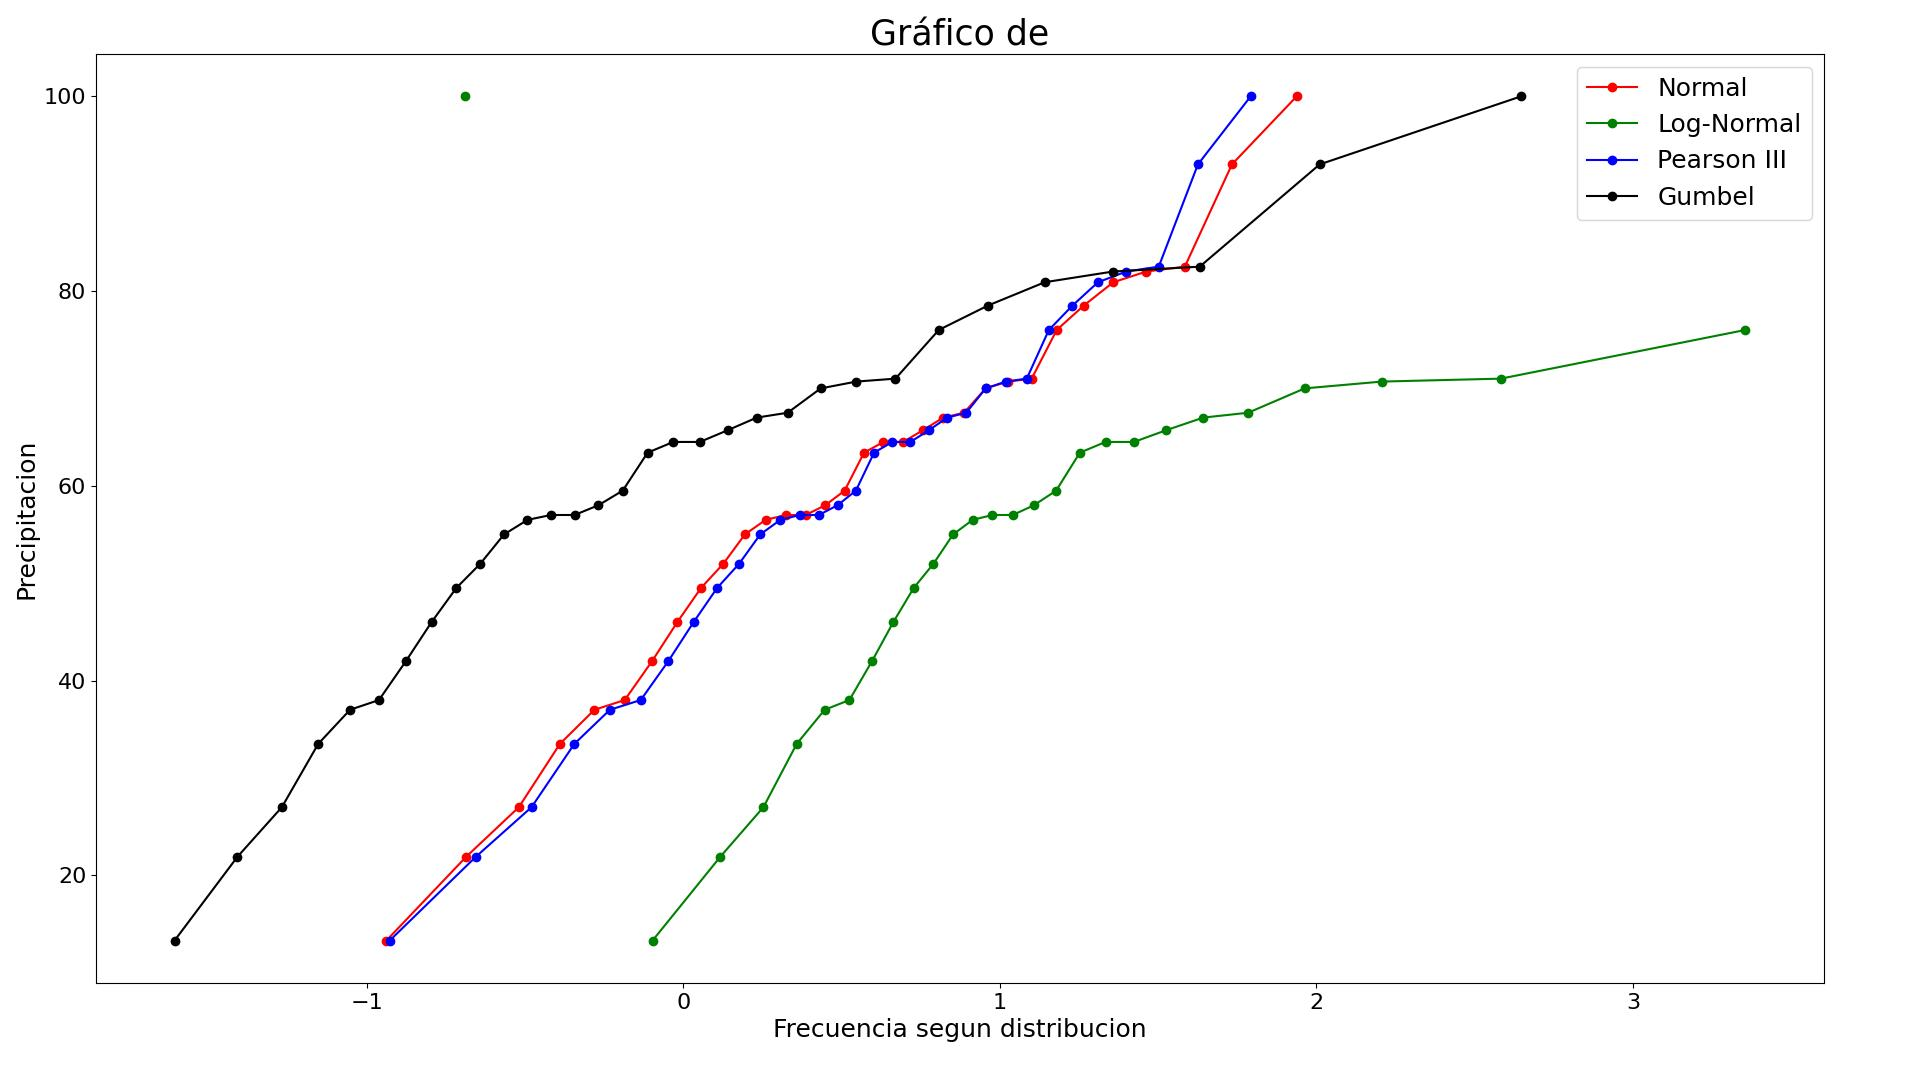
\includegraphics[width=0.8\textwidth]{grafico.jpg}
    \caption{Precipitaciones máximas diarias historicas en la estación de San José de Maipo}
    \label{fig:precipitaciones_maximas_diarias}
\end{figure}

\newpage
\subsubsection{Parte B}

Luego se muestra un grafico con las precipitaciones máximas diarias en la estación de San José de Maipo, con las proyecciones futuras para el año 2040 hasta 2069.

\begin{figure}[H]
    \centering
    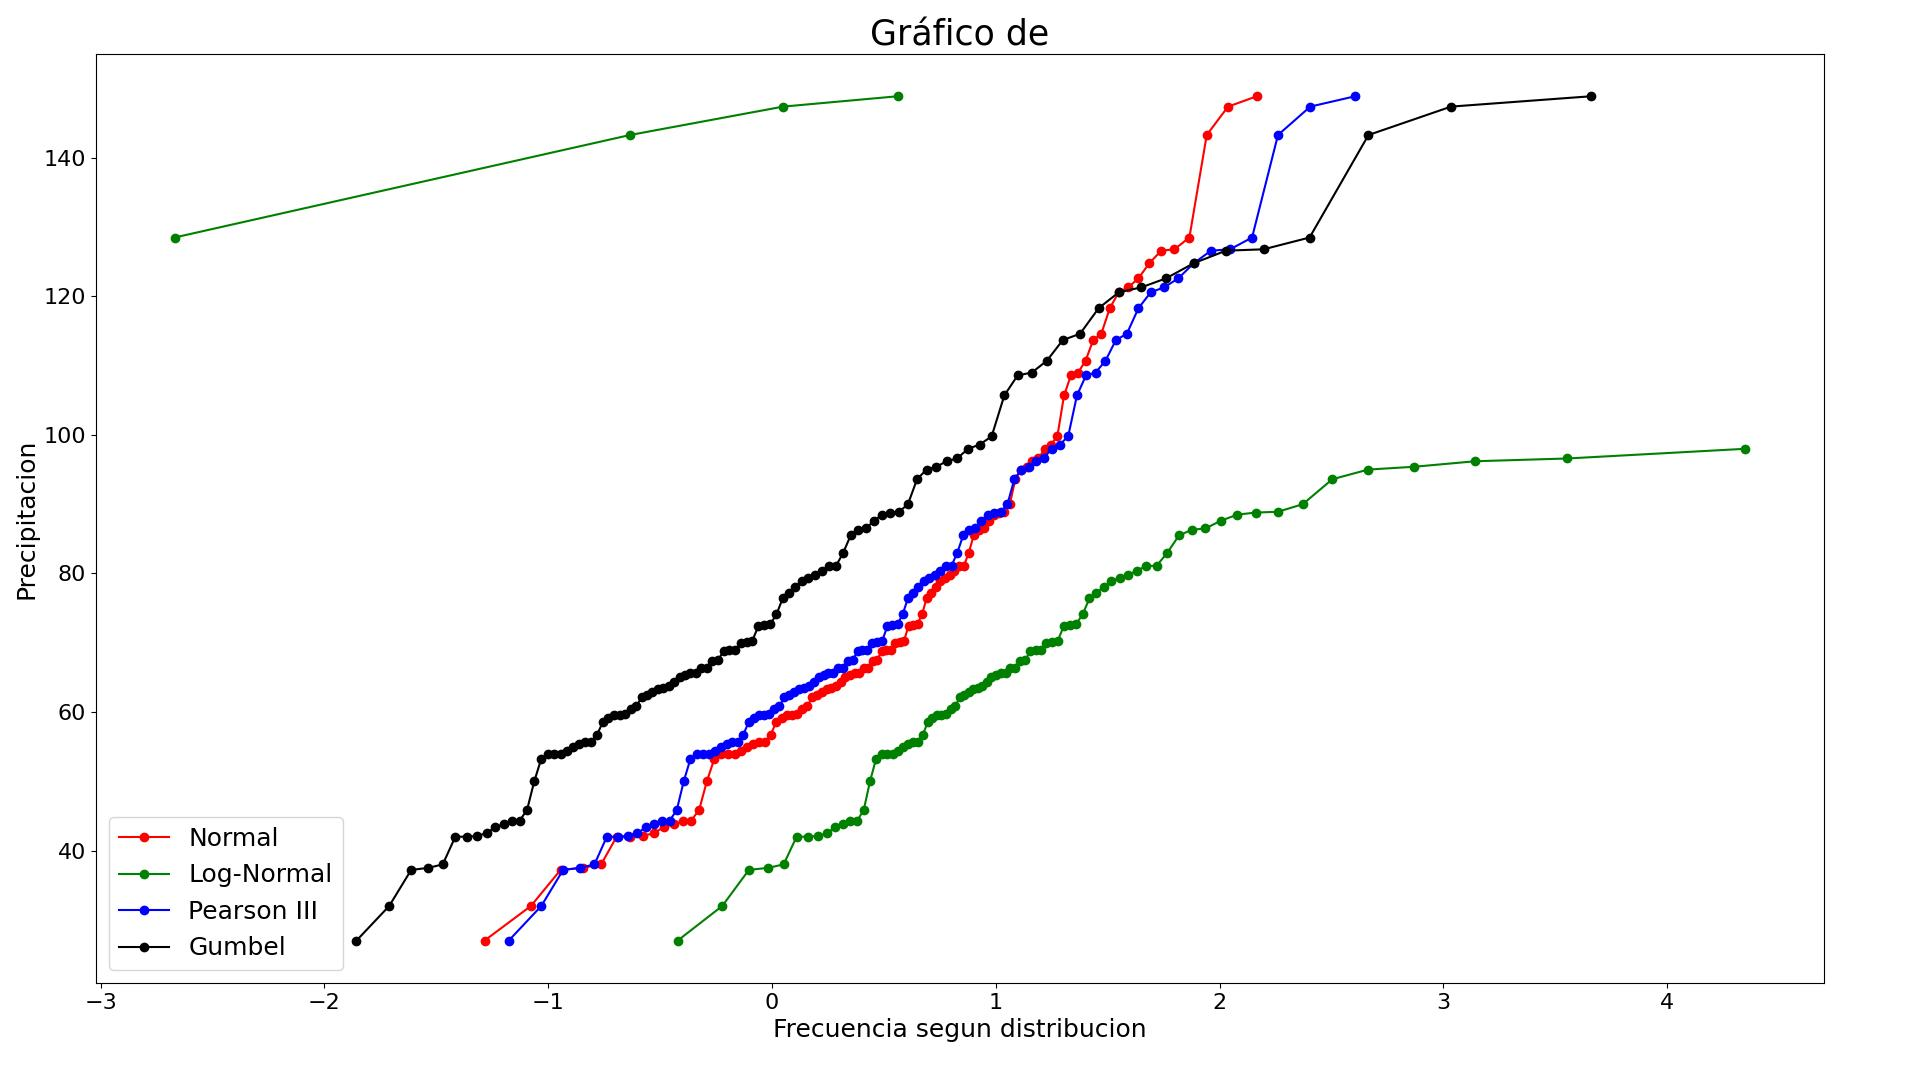
\includegraphics[width=0.8\textwidth]{grafico_b.jpg}
    \caption{Precipitaciones máximas diarias proyectadas a futuro en la estación de San José de Maipo}
    \label{fig:precipitaciones_maximas_diarias}
\end{figure}


\subsubsection{Parte C}




\end{document}
